\begin{figure}[h!]

  % Define the layers to draw the diagram
  \pgfdeclarelayer{background}
  \pgfsetlayers{background,main}

  % Define a new shape: page with a folded corner 
  \makeatletter
  \pgfdeclareshape{flippedpage}{
    \inheritsavedanchors[from=rectangle] % this is nearly a rectangle
    \inheritanchorborder[from=rectangle]
    \inheritanchor[from=rectangle]{center}
    \inheritanchor[from=rectangle]{north}
    \inheritanchor[from=rectangle]{south}
    \inheritanchor[from=rectangle]{west}
    \inheritanchor[from=rectangle]{east}
    % ... and possibly more
    \backgroundpath{% this is new
    % store lower left in xa/ya and upper right in xb/yb
    \southwest \pgf@xa=\pgf@x \pgf@ya=\pgf@y
    \northeast \pgf@xb=\pgf@x \pgf@yb=\pgf@y
    % compute corner of ``flipped page''
    \pgf@xc=\pgf@xb \advance\pgf@xc by-5pt % this should be a parameter
    \pgf@yc=\pgf@yb \advance\pgf@yc by-5pt
    % diagonal path of the corner 
    \pgfpathmoveto{\pgfpoint{\pgf@xa}{\pgf@ya}}
    \pgfpathlineto{\pgfpoint{\pgf@xa}{\pgf@yb}}
    \pgfpathlineto{\pgfpoint{\pgf@xc}{\pgf@yb}}
    \pgfpathlineto{\pgfpoint{\pgf@xb}{\pgf@yc}}
    \pgfpathlineto{\pgfpoint{\pgf@xb}{\pgf@ya}}
    \pgfpathclose
    % add little corner
    \pgfpathmoveto{\pgfpoint{\pgf@xc}{\pgf@yb}}
    \pgfpathlineto{\pgfpoint{\pgf@xc}{\pgf@yc}}
    \pgfpathlineto{\pgfpoint{\pgf@xb}{\pgf@yc}}
    \pgfpathlineto{\pgfpoint{\pgf@xc}{\pgf@yc}}
    }
  }

  % Define block styles
  \tikzstyle{plugin}=[draw, fill=white, text width=0.9cm, text centered,
  minimum height=0.9cm, rounded corners=1]
  \tikzstyle{specialplugin}=[draw, fill=blue!20, text width=0.9cm, text centered,
  minimum height=0.9cm, rounded corners=1]
  \tikzstyle{code}=[draw,shape=flippedpage,text width=0.6cm, text centered, minimum height=2.6em,fill=white]
\tikzstyle{texttitle}=[fill=white, rounded corners=1, draw=black!50]%, dashed]
\tikzstyle{background}=[rounded corners=1, draw=black!50]%, dashed]

  \begin{center}
  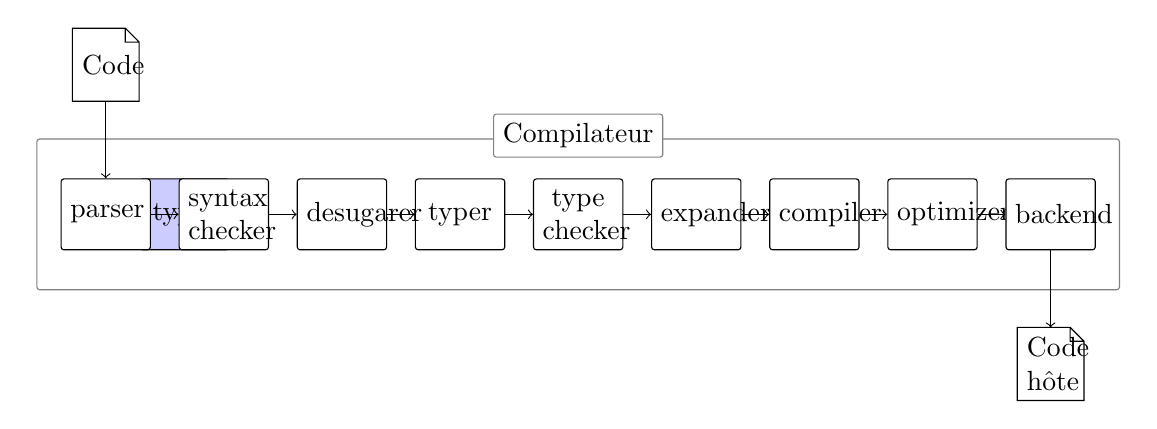
\begin{tikzpicture}%[scale=0.9]
	  % Draw diagram elements
	  \node (typechecker) [plugin] {\minicode{type checker}};
	  %\path (typechecker.west) node (arrowt-tc) [arrow] {};
	  \path (typechecker)+(-5,0.0) node (transformer) [specialplugin]
	  {\minicode{typer}};
	  \path (typechecker)+(-1.5,0.0) node (typer) [plugin]
	  {\minicode{typer}};
	  %\path (typer.west) node (arrowd-t) [arrow] {};
	  \path (typechecker)+(-3.0,0.0) node (desugarer) [plugin] {\minicode{desugarer}};
	  %\path (desugarer.west) node (arrowsc-d) [arrow] {};
	  \path (typechecker)+(-4.5,0.0) node (syntaxchecker) [plugin]
	  {\minicode{syntax checker}};
	  %\path (syntaxchecker.west) node (arrowp-sc) [arrow] {};
	  \path (typechecker)+(-6.0,0.0) node (parser) [plugin]
	  {\minicode{parser}};
	  %\path (parser.west) node (inputarrow) [bigarrow] {};
	  \path (typechecker)+(-6.0,1.9) node (tomfile) [code]
    {\minicode{Code {\tom}}};

	  \path (typechecker)+(1.5,0.0) node (expander) [plugin]
	  {\minicode{expander}};
	  \path (typechecker)+(3.0,0.0) node (compiler) [plugin]
	  {\minicode{compiler}};
	  \path (typechecker)+(4.5,0.0) node (optimizer) [plugin]
	  {\minicode{optimizer}};
	  \path (typechecker)+(6.0,0.0) node (backend) [plugin]
	  {\minicode{backend}};
	  \path (typechecker)+(6.0,-1.9) node (javafile) [code]
    {\minicode{Code hôte}};

	  % Draw arrows between elements
	  \path [draw, ->] (tomfile.south) -- node [left] {} (parser);
%	  \path [draw, ->] (parser.south) -- node [left] {} (transformer);
%	  \path [draw, ->] (transformer.east) -- node [above] {} (syntaxchecker);
	  \path [draw, ->] (parser.east) -- node [above] {} (syntaxchecker);
	  \path [draw, ->] (syntaxchecker.east) -- node [above] {} (desugarer);
	  \path [draw, ->] (desugarer.east) -- node [above] {} (typer);
	  \path [draw, ->] (typer.east) -- node [above] {} (typechecker);
	  \path [draw, ->] (typechecker.east) -- node [above] {} (expander);
	  \path [draw, ->] (expander.east) -- node [above] {} (compiler);
	  \path [draw, ->] (compiler.east) -- node [above] {} (optimizer);
	  \path [draw, ->] (optimizer.east) -- node [above] {} (backend);
	  \path [draw, ->] (backend.south) -- node [above] {} (javafile);

	  % Draw layer titles
	  \path (typechecker)+(0.0,1.0) node (tomtitle) [texttitle]
    {\figcode{Compilateur {\tom}}};
		  

	  % Draw background
	  \begin{pgfonlayer}{background}
	  % Left-top corner of the background rectangle
	  \path (parser.west |- parser.north)+(-0.3,0.5) node (a) {};
	  % Right-bottom corner of the background rectangle
	  \path (backend.east|- backend.south)+(0.3,-0.5) node (b) {};

	  % Draw the background
	  \path[background]
	  (a) rectangle (b);
	  \end{pgfonlayer}
  \end{tikzpicture}
  \end{center}
  \caption{Modules of the {\tom} system.}
\label{fig:architecture}
\end{figure}
